\documentclass[]{report}

\usepackage[utf8]{inputenc}
\usepackage[spanish]{babel}

\usepackage{graphicx}
\usepackage{listings}
\usepackage{hyperref}

% Title Page
\title{PECL2 - Algoritmos Voraces}
\author{Jorge Guillamón y Miguel Ángel Guerrero}


\begin{document}
\maketitle

\begin{abstract}
	Se describen los algoritmos de los ejercicios 2, 3, 5, 6. Todos los códigos fuente se pueden encontrar en este mismo directorio.
\end{abstract}

\subsection*{Ejercicio 2 - Almacenamiento de ficheros en el disco duro}
Hemos considerado que el parámetro a maximizar debe ser el número de accesos por byte del archivo. De esta manera, se colocarán en primera posición los archivos más accedidos y pequeños y al final los menos accedidos y pesados.\\
Hemos aprovechado las facilidades que da Python para resolver el problema en 2 líneas.
\begin{figure}[h!]
	\centering
	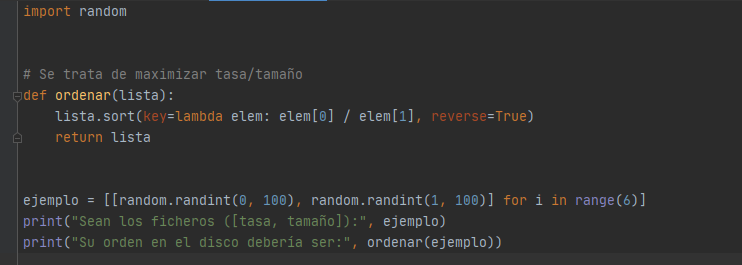
\includegraphics[width=1\linewidth]{1}
	\caption{}
	\label{fig:1}
\end{figure}

Como se puede apreciar, el probador cambia para cada ejecución.
\newpage

\subsection*{Ejercicio 3 - Mínimo y máximo de una lista}

En este caso, lo principal es diseñar un algoritmo eficaz teniendo siempre en cuenta el número de comparaciones que va a realizar, ya que un mínimo y máximo se puede programar de muchas maneras, pero para que cumpla con una eficacia menor a 3/2N hemos tenido que pensar de forma un poco diferente a lo habitual. El algoritmo diseñado sigue cumpliendo las características básicas de los algoritmos voraces, algo que facilita el mismo diseño de este y nos muestra su utilidad.\\\\
Como entrada requiere una lista, de la cual obtenemos su longitud. La longitud de esta es clave para el desarrollo. Si se da un número de elementos totales pares, el bucle, que comentamos más adelante, empieza con (i=2), y por el contrario, con (i=1).\\\\
A partir de esta parte, pasa al bucle, el cual recorre la lista de números desde su principio, comparando uno a uno, con el siguiente cual es el máximo y cual es el mínimo de manera que los va actualizando en el caso de que A)exista máximo B)exista mínimo, sino, mantendría valores. Si por ejemplo tenemos una Lista [1,2,3]:\\
El máximo y mínimo se establece al valor en [0].\\\\
Entra al While, desde i=1. Si el elemento en [1] es menor que el siguiente elemento, el mínimo, es el mínimo entre el menor número que ya había, y ese número menor en [1].\\\\
De esta forma nos aseguramos de que el mínimo siempre irá a menos y el máximo siempre irá más, y como algoritmo voraz, recorre todas las opciones valorando estas posibilidades.\\\\
Para el caso de N elementos impares el número de comparaciones llega a ser : 3*(n-1)/2  
Si por el contrario, se da que N es de la forma 2*N;\\
\begin{itemize}
	\item Debemos de inicializar el máximo y el mínimo haciendo una primera comparación de los 2 primeros elementos, a esto le sumamos 3(n-2)/2 comparaciones para el resto de los elementos de la lista. SI despejamos 1 + 3*(N-2)/2 nos queda el resultado en cualquiera de los casos es menor a 3/2 N, que es 3n/2 -2
\end{itemize}\newpage

\begin{figure}[h!]
	\centering
	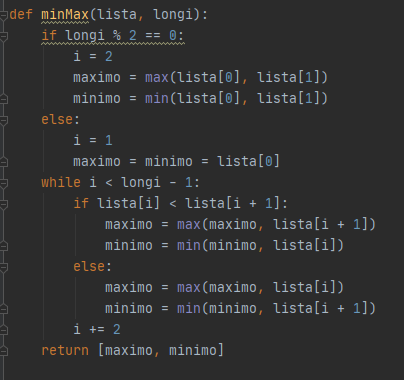
\includegraphics[width=0.65\linewidth]{6}
	\caption{}
	\label{fig:6}
\end{figure}\newpage

\newpage
\subsection*{Ejercicio 5 - Dijkstra}
Se he implementado un algoritmo de Dijkstra aunque usando estructuras de datos en lugar de matrices para almacenar las distancias mínimas.\\
\begin{figure}[h!]
	\centering
	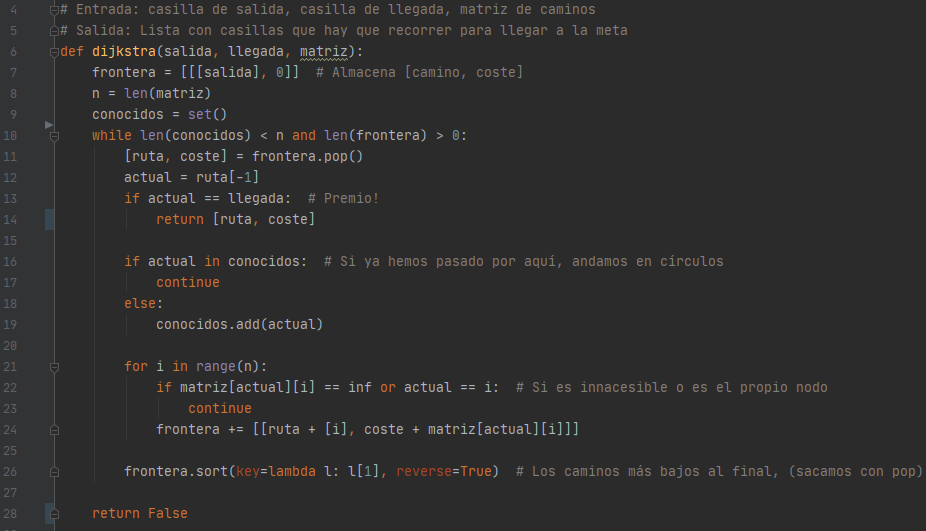
\includegraphics[width=1\linewidth]{2}
	\caption{}
	\label{fig:2}
\end{figure}\\
En este sentido, los elementos de la frontera del algoritmo almacenan [ruta hasta ese momento, coste asociado]. Al final de cada iteración se ordena la frontera de acuerdo al algoritmo original.\\\\
El código está listo para ser probado con 2 matrices de ejemplo. Una vez ejecutado el programa, aparecerá por pantalla el camino más corto junto con su coste.
\begin{figure}[h!]
	\centering
	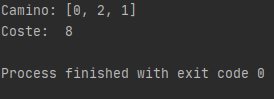
\includegraphics[width=0.4\linewidth]{3}
	\caption{}
	\label{fig:3}
\end{figure}
\newpage
\subsection*{Ejercicio 6 - Shrek y las escaleras}
La solución que hemos planteado consiste en elegir los 2 tramos de escalera más pequeños disponibles en cada iteración. Tras acabar la iteración, se añade el nuevo tramo a la lista de los diponibles y se eliminan los usados.\\
\begin{figure}[h!]
	\centering
	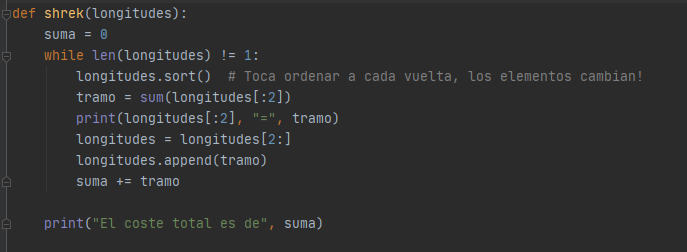
\includegraphics[width=1\linewidth]{4}
	\caption{}
	\label{fig:4}
\end{figure}\\
La salida es por pantalla, en primer lugar se mostrarán los tramos disponibles. Durante la ejecución del algoritmo, cuando se vayan a fundir dos tramos se indicarán cuales son, finalmente se indicará el coste total.

El ejercicio viene acompañado de un probador que cambia para cada ejecución.
\begin{figure}[h!]
	\centering
	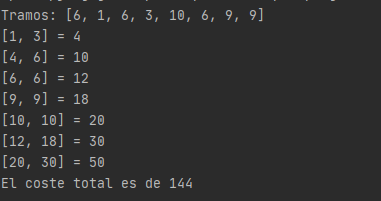
\includegraphics[width=0.7\linewidth]{5}
	\caption{}
	\label{fig:5}
\end{figure}



\end{document}          
